\documentclass[10pt]{exam}
\usepackage[hon]{template-for-exam}
\usepackage{tikz}
\usetikzlibrary{
  calc,
  patterns,
  decorations.pathmorphing,
}





\title{Energy in Simple Harmonic Oscillators}
\author{Rohrbach}
\date{\today}

\begin{document}
\maketitle

\noindent
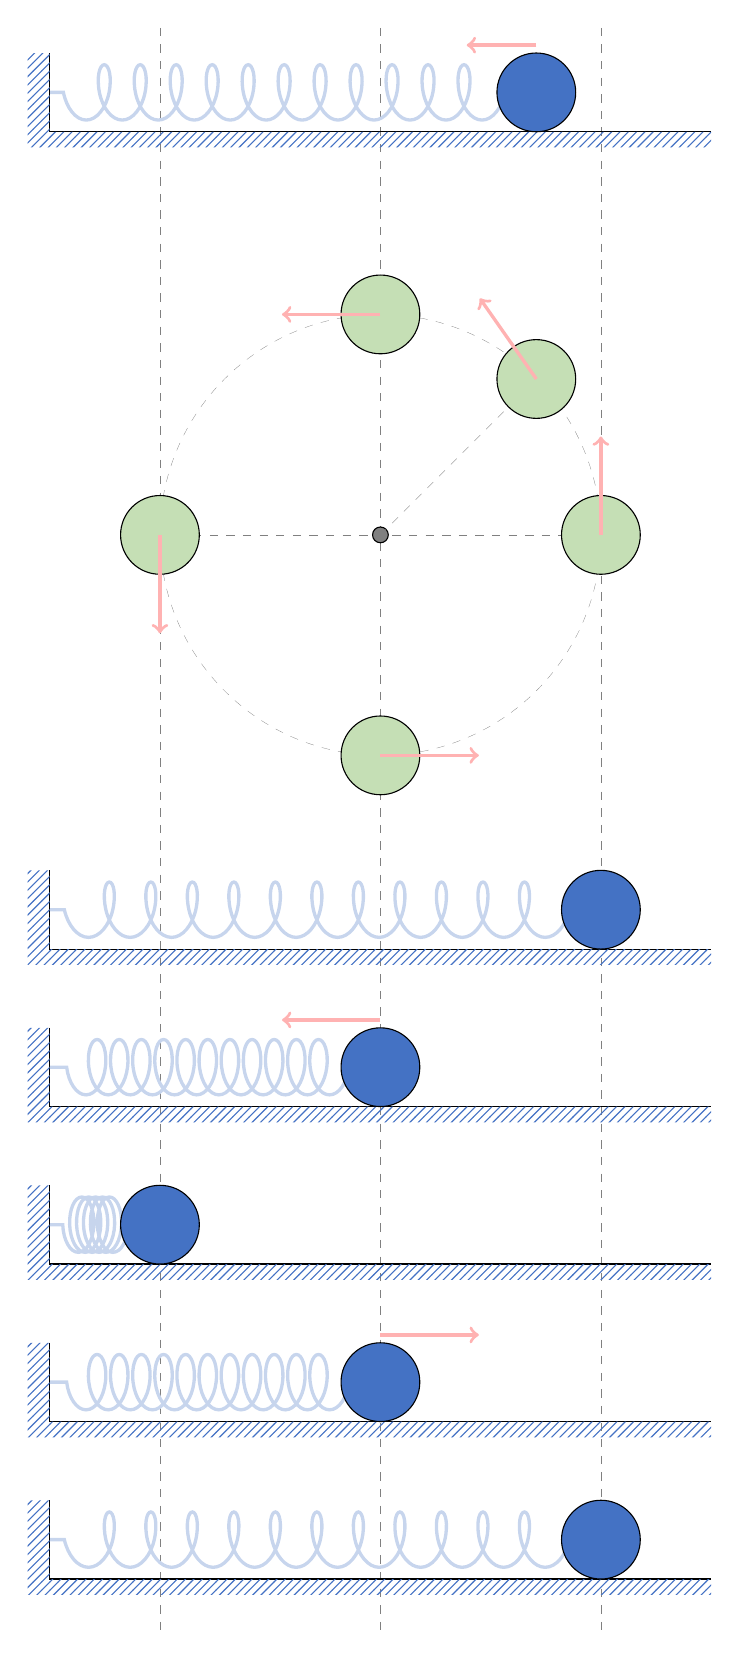
\begin{tikzpicture}
  \def\amp{2.8}
  \def\massradius{.5}
  \def\sep{2}
  \def\ceilingheight{2*\amp}
  \def\startofspring{1.7*\amp}
  \def\endofpicx{\startofspring+3.5*\sep}
  \def\endofpicy{-14}
  \def\springending{.1}
  \def\veclength{1.25}
  \def\leftanchor{-1.5*\amp}

  \definecolor{springcolor}{HTML}{4472C4}
  \definecolor{circlecolor}{HTML}{C5DFB5}

  \tikzstyle{guides}=[
      ultra thin,
      gray,
      dashed
    ]
  \tikzstyle{cmass}=[
      radius=\massradius,
      fill=circlecolor
    ]
  \tikzstyle{smass}=[
      radius=\massradius,
      fill=springcolor,
    ]
  \tikzstyle{ceiling}=[
      pattern=north east lines,
      pattern color=springcolor
    ]
  \tikzstyle{spring}=[
      very thick,
      springcolor!30,
      decoration={
        coil,
        amplitude=10
      }
    ]
  \tikzstyle{vector}=[
      red!30,
      very thick,
      ->
    ]

  \coordinate (ceiling start) 
                  at (\leftanchor, -0.5*\amp);
  \coordinate (ceiling end)   
                  at (\leftanchor, \endofpicy);
  %\fill[ceiling] (ceiling start) -- (ceiling end)
  %   -- ++(-.5,0) |- cycle;
  %\draw (ceiling start) -- (ceiling end) -- ++ (-0.5,0);

  \draw[guides] (-\amp, 2.3*\amp) -- (-\amp, \endofpicy);
  \draw[guides] ( \amp, 2.3*\amp) -- ( \amp, \endofpicy);
  \draw[guides] (0    , 2.3*\amp) -- (0    , \endofpicy);
  \draw[guides] (-\amp, 0   ) -- (\amp , 0         );


  \coordinate (ccenter) at (0,0);
  \filldraw[fill=gray] (ccenter) circle[radius=0.1];
  \draw[guides]        (ccenter) circle[radius=\amp];


  \coordinate (c1) at (  0:\amp);
  \coordinate (c2) at ( 45:\amp);
  \coordinate (c3) at ( 90:\amp);
  \coordinate (c4) at (180:\amp);
  \coordinate (c5) at (270:\amp);
  
  \draw[guides] (ccenter) -- (c2);

  \foreach \x in {(c1),(c2),(c3),(c4),(c5)} {
    \draw[cmass] \x circle;
  }

  \draw[vector] (c1) -- ++( 90:\veclength);
  \draw[vector] (c2) -- ++(125:\veclength);
  \draw[vector] (c3) -- ++(180:\veclength);
  \draw[vector] (c4) -- ++(270:\veclength);
  \draw[vector] (c5) -- ++(  0:\veclength);



  \path[smass] (ccenter) 
    ++(\amp ,-\startofspring) coordinate (s1)
    ++(-\amp,  -\sep) coordinate (s3)
    ++(-\amp,  -\sep) coordinate (s4)
    ++(\amp ,  -\sep) coordinate (s5)
    ++(\amp ,  -\sep) coordinate (s6);



  %usage \drawspring{(location of mass)}{segment length}
  \newcommand{\drawspring}[2]{
    \coordinate (thismass) at #1;
    \coordinate (top) at 
      (ceiling start |- thismass);
    \draw[spring,segment length=#2] (thismass)
      -- ++ (-\massradius+\springending,0) 
      decorate {-- ($(top) + (\springending,0)$) }
      -- (top);
    \draw (top) +(0,0.5) -- ++(0,-0.5) -- ++(3*\amp,0);
    \fill[ceiling] 
      (top) +(0,0.5) -- ++(0,-0.5) -- ++(3*\amp,0)
      -- ++(0,-0.2) -- ++(-3.1*\amp,0) 
      -- ++(0,1.2) -- cycle;
  }

  \drawspring{(s1)}{15}
  \draw[smass] (s1) circle;

  \drawspring{(s3)}{8}
  \draw[smass] (s3) circle;
  \draw[vector] (s3) ++(0,.6) -- ++ (-\veclength,0);

  \drawspring{(s4)}{2.5}
  \draw[smass] (s4) circle;

  \drawspring{(s5)}{8}
  \draw[smass] (s5) circle;
  \draw[vector] (s5) ++(0,.6) -- ++ (\veclength,0);


  \drawspring{(s6)}{15}
  \draw[smass] (s6) circle;


  \path[smass] (c2) 
    ++ (0,1.3*\amp) coordinate (s2);
  \drawspring{(s2)}{13}
  \draw[smass] (s2) circle;
  \draw[vector] (s2) ++(0,.6) -- ++ (-0.707*\veclength,0);


\end{tikzpicture}

\pagebreak

\section*{Practice}

%\begin{questions}

%\question
  A 0.60-kg mass is placed on a spring and set to oscillate with an amplitude of 13~cm.  Its frequency is 4.0~Hz.

  \vspace{1em}

  \begin{parts}
    \part
      Calculate the maximum speed of the mass.
    \part
      How fast is the mass moving when its displacement from equilibrium is 9~cm?
    \part
      Write down the equation for motion of the mass.
  \end{parts}

  \vs[3]

% \question 
%   An object of mass 0.75~kg oscillates according to the equation $x(t)=0.45\cos\left(6.40 \cdot t\right)$, where $x$ is measured in meters and $t$ is measured in seconds.


%   \begin{parts}
%     \part
%       What is the amplitude?
%     \part
%       What is the frequency?
%     \part
%       What is the total energy of the system?
%   \end{parts}

%   \vs



  
% \end{questions}



\end{document}